\documentclass{article}

% if you need to pass options to natbib, use, e.g.:
%     \PassOptionsToPackage{numbers, compress}{natbib}
% before loading neurips_2024


% ready for submission
\usepackage[preprint]{main}


% to compile a preprint version, e.g., for submission to arxiv, add add the
% [preprint] option:
%     \usepackage[preprint]{neurips_2024}


% to compile a camera-ready version, add the [final] option, e.g.:
%     \usepackage[final]{neurips_2024}


% to avoid loading the natbib package, add option nonatbib:
%    \usepackage[nonatbib]{neurips_2024}


\usepackage[utf8]{inputenc} % allow utf-8 input
\usepackage[T1]{fontenc}    % use 8-bit T1 fonts
\usepackage{url}            % simple URL typesetting
\usepackage{booktabs}       % professional-quality tables
\usepackage{amsfonts}       % blackboard math symbols
\usepackage{nicefrac}       % compact symbols for 1/2, etc.
\usepackage{microtype}      % microtypography
\usepackage{xcolor}         % colors
\usepackage{graphicx}	%image
\usepackage{amsmath, nccmath}	%align
\usepackage{tikz}
\usepackage[fleqn,tbtags]{mathtools}
\usepackage{cancel}
\usepackage[mathscr]{euscript}
\usepackage{tabto}
\usepackage{mathtools}
\usepackage{graphicx}
\usepackage{setspace}
\usepackage[fontsize=12pt]{scrextend}
\usepackage{bigints}

\DeclarePairedDelimiterX{\infdivx}[2]{(}{)}{%
  #1\;\delimsize\|\;#2%
}
\newcommand{\infdiv}{D_{KL}\infdivx}
\newcommand*{\Scale}[2][4]{\scalebox{#1}{\ensuremath{#2}}}

% https://www.overleaf.com/read/wzwnrbbwrvyx
% https://tex.stackexchange.com/questions/162207/algorithm2e-comment-style
% https://tex.stackexchange.com/questions/298339/how-to-insert-a-continue-in-while-command-of-algorithm2e
% https://tex.stackexchange.com/questions/195991/aligning-in-and-out-text-for-algorithms
% https://tex.stackexchange.com/questions/155542/algorithm-write-if-then-return-or-else-return-in-one-line
\usepackage[linesnumbered,ruled,vlined]{algorithm2e}

% https://tex.stackexchange.com/questions/200730/how-to-have-the-algorithmicx-comment-symbol-in-algorithm2e
\SetKwComment{Comment}{$\triangleright$\ }{}
% \newcommand\mycommfont[1]{\footnotesize\ttfamily\textcolor{black}{#1}}
% \SetCommentSty{mycommfont}

\SetKwInput{KwInput}{Input}                % Set the Input
\SetKwInput{KwOutput}{Output}              % set the Output

\SetKw{Andd}{and} % `\And` already exists
\SetKw{Break}{break}
\SetKw{Continue}{continue}
\SetKw{Return}{return}

% https://english.stackexchange.com/questions/338/when-is-l-doubled

% \newcommand{\all}{\textbf{all}~}

\newcommand{\both}{\textbf{both}~}
    \newcommand{\andd}{\textbf{and}~}

\newcommand{\butalso}{\textbf{but also~}}
    \newcommand{\notonly}{\textbf{not only~}}

\newcommand{\cf}{cf.~}

\newcommand{\eg}{e.g.~}
\newcommand{\either}{\textbf{either~}}
    \newcommand{\orr}{\textbf{or}~}
% \newcommand{\every}{\textbf{every~}}

\newcommand{\first}{\textbf{Firstly},~}
    \newcommand{\second}{\textbf{Secondly},~}
    \newcommand{\third}{\textbf{Third},~}
    \newcommand{\fourth}{\textbf{Fourth},~}
    \newcommand{\final}{\textbf{Finally},~}
    \newcommand{\last}{\textbf{Lastly},~}

% \newcommand{\from}{\textbf{from}~}
%     \newcommand{\tob}{\textbf{to}~}

% \newcommand{\never}{\textbf{never}~}
% \newcommand{\no}{\textbf{no}}
\newcommand{\nott}{\textbf{not}~}

\newcommand{\ie}{i.e.~}
\newcommand{\incl}{incl.~} % https://dictionary.cambridge.org/dictionary/english/incl
\newcommand{\iiddot}{i.i.d}
% \newcommand{\iid}{\iiddot~} % many tildes may cause compile error, eg in `~\iid`
\newcommand{\st}{s.t.~}
\newcommand{\vs}{vs.~}

\newcommand{\orrr}{\textbf{or}~}

\newcommand{\wrt}{with respect to~}

% https://tex.stackexchange.com/questions/57152/how-to-draw-graphs-in-latex
% https://tex.stackexchange.com/questions/300098/draw-a-node-as-a-square-with-tikz
% https://tex.stackexchange.com/questions/350049/tikz-pgfplots-how-to-make-tikzpcture-fit-the-parent-figure-subfigure-float-envi/
% https://rmwu.github.io/tutorial/latex/2019/11/21/positioning/
% https://texample.net/tikz/examples/
\usepackage{tikz}
\usetikzlibrary{positioning, shapes.geometric, backgrounds}
% \usetikzlibrary{positioning, shapes, shadows, arrows}

% https://tex.stackexchange.com/questions/5461/is-it-possible-to-change-the-size-of-an-arrowhead-in-tikz-pgf/161238#161238
% https://tex.stackexchange.com/questions/409881/self-loop-arrowhead-different-cannot-change
% https://github.com/pgf-tikz/pgf/issues/1008
    % [>={Arrowtype}] this means "make all arrows {ArrowType}" and you supply this to generic style settings.
    % [-{Arrowtype}] this means "put an end arrow head {ArrowType}" and you supply this style to paths and edges
\usetikzlibrary{arrows.meta}

% https://tex.stackexchange.com/questions/13625/subcaption-vs-subfig-best-package-for-referencing-a-subfigure
% https://tex.stackexchange.com/questions/333249/controlling-subfigure-captions-and-subfigure-placement
% https://tex.stackexchange.com/questions/13150/subfigures-with-tikz-on-the-same-line
% http://www.peteryu.ca/tutorials/publishing/latex_captions
% \usepackage{subfigure} % clash with `subcaption`
% \usepackage{subfig}
\usepackage{subcaption}

% https://tex.stackexchange.com/questions/110513/unknown-graphics-extension-1-png
\usepackage{grffile}

% https://tex.stackexchange.com/questions/8532/is-eps-or-pdf-the-preferred-figure-format-when-typesetting-in-latex
% https://tex.stackexchange.com/questions/45498/choosing-whether-to-include-pdf-or-png-in-pdflatex
% https://www.overleaf.com/learn/latex/Managing_images
% https://www.overleaf.com/learn/how-to/Why_do_I_keep_getting_the_compile_timeout_error_message%3F
\usepackage{graphicx} % Allows including images
\DeclareGraphicsExtensions{.pdf,.jpeg,.png,.jpg}

% https://tex.stackexchange.com/questions/50070/landscape-figure-in-latex
% https://tex.stackexchange.com/questions/37600/how-to-rotate-a-group-of-figures-subfigure
% https://tex.stackexchange.com/questions/471472/how-to-make-figures-appear-landscape-properly
% https://tex.stackexchange.com/questions/438798/how-to-get-landscape-float-with-correct-numbering
% https://tex.stackexchange.com/questions/159988/sidewaysfigure-and-landscape
\usepackage{rotating}

% https://www.overleaf.com/learn/latex/wrapping_text_around_figures
% https://tex.stackexchange.com/questions/31764/white-space-under-wrapfigure-caption
\usepackage{wrapfig}

% https://tex.stackexchange.com/questions/15971/bibliography-with-page-numbers
% \usepackage[hidelinks, bookmarksnumbered]{hyperref}
\usepackage[hidelinks, bookmarksnumbered, backref=page]{hyperref}
\renewcommand*{\backref}[1]{}
\renewcommand*{\backrefalt}[4]{
  \ifcase #1 (Broken backref)
  \or        (page~#2)
  \else      (pages~#2)
  \fi
}

\hypersetup{
  colorlinks   = true,
  urlcolor     = blue,
  linkcolor    = blue,
  citecolor   = blue
}

\usepackage{url}            % simple URL typesetting

% https://tex.stackexchange.com/questions/36175/what-do-newcommand-renewcommand-and-providecommand-do-and-how-do-they-differ
% https://tex.stackexchange.com/questions/163280/underbar-changing-the-style-of-font-but-bar-not-why

% https://tex.stackexchange.com/questions/341717/smaller-font-for-subscript-within-subscript-in-math-mode
\usepackage{scalerel}
\usepackage{amsmath}
\usepackage{amsthm}
\usepackage{amssymb}
\usepackage{amsfonts}       % blackboard math symbols
\usepackage{mathtools}
\usepackage{cancel}
\usepackage{bbm} % for `\mathbbm{b}`

% https://tex.stackexchange.com/questions/479/lowercase-mathcal
\usepackage{dutchcal}

% https://tex.stackexchange.com/questions/118173/how-to-write-ceil-and-floor-in-latex
\usepackage{mathtools}
\DeclarePairedDelimiter\ceil{\lceil}{\rceil}
\DeclarePairedDelimiter\floor{\lfloor}{\rfloor}

% Math operator macros %%%%%%%%%%%%%%%%%%%%%%%%%%%%%%%%%%%%%%%%%%%%%%%%%%%%%%%%%
\newcommand{\abs}[1]{\left|#1\right|}
\newcommand{\clip}{\mathrm{clip}}
\newcommand{\cov}[1]{\mathrm{Cov}(#1)}
\newcommand{\diag}{\mathrm{diag}}

\newcommand{\E}[2]{\mathbb{E}_{#1} \left[ #2 \right]} % expectation

\newcommand{\interior}[1]{\mathrm{interior}(#1)}

\newcommand{\norm}[1]{\|#1\|} % for ordinary vectors
\newcommand{\normm}[1]{\left\|#1\right\|}
\newcommand{\nullspace}{\mathrm{Null}}

\newcommand{\partdiff}[1]{\frac{\partial}{\partial #1}}
\newcommand{\partdiffb}[2]{\frac{\partial #2}{\partial #1}}

\newcommand{\rank}{\mathrm{rank}}

\newcommand{\ud}{\mathrm{d}}

\newcommand{\prob}[1]{\mathrm{Pr}\{#1\}}

\newcommand{\realset}{\mathbb{R}}
\newcommand{\real}[1]{\mathbb{R}^{#1}}
\newcommand{\integer}[1]{\mathbb{Z}^{#1}}
\newcommand{\naturall}[1]{\mathbb{N}^{#1}}

\newcommand{\set}[1]{\left\{ #1 \right\}}
\newcommand{\setname}[1]{\mathcal{#1}}
\newcommand{\setsize}[1]{|\mathcal{#1}|}
\newcommand{\setsizesubt}[1]{|\mathcal{#1}_t|}
\newcommand{\setsizesubx}[2]{|\mathcal{#1}_{#2}|}

% http://statweb.stanford.edu/~owen/courses/363/scribe_template.tex
\newcommand{\simiid}{\stackrel{\mathrm{iid}}{\sim}}

% https://tex.stackexchange.com/questions/111544/what-is-the-capital-greek-letter-for-tau
\newcommand{\Tau}{\mathrm{T}}
\newcommand{\trace}{\mathrm{trace}}
\newcommand{\var}{\mathrm{var}}

\newcommand{\spanspace}{\mathrm{span}}

\newcommand{\eqset}{\mathrel{\overset{\makebox[0pt]{\mbox{\normalfont\tiny\sffamily set}}}{=}}}

% https://tex.stackexchange.com/questions/4216/how-to-typeset-correctly
% \newcommand{\eqdef}{\mathrel{\overset{\makebox[0pt]{\mbox{\normalfont\tiny\sffamily def}}}{=}}}
\newcommand{\eqdef}{\coloneqq}
\newcommand{\eqdefr}{\eqqcolon}

\newcommand{\widebar}[1]{\overline{#1}}
\DeclareMathOperator*{\argmin}{\arg\!\min}
\DeclareMathOperator*{\argmax}{\arg\!\max}
\renewcommand\qedsymbol{$\blacksquare$}

% `\mathbf{}` does not work for eg \hat{\mat{}}
\newcommand{\vecb}[1]{\boldsymbol{#1}}
\newcommand{\mat}[1]{\boldsymbol{#1}}

% https://tex.stackexchange.com/questions/2607/spacing-around-left-and-right/
\let\originalleft\left
\let\originalright\right
\renewcommand{\left}{\mathopen{}\mathclose\bgroup\originalleft}
\renewcommand{\right}{\aftergroup\egroup\originalright}

\newtheorem{theorem}{Theorem}[section]
\newtheorem{corollary}{Corollary}[theorem]
\newtheorem{definition}{Definition}[section]
\newtheorem{lemma}{Lemma}[section]
\newtheorem{proposition}{Proposition}[section]
\newtheorem{assumption}{Assumption}[section]
\newtheorem{remark}{Remark}[section]

% MDP special states and actions %%%%%%%%%%%%%%%%%%%%%%%%%%%%%%%%%%%%%%%%%%%%%%%
\newcommand{\szrat}{s_{\mathrm{zrat}}} % zrat: zero reward absorbing terminal
\newcommand{\azrat}{a_{\mathrm{zrat}}}
\newcommand{\pzrat}{p_{\mathrm{zrat}}}
\newcommand{\rzrat}{r_{\mathrm{zrat}}}
\newcommand{\isdzrat}{\isd_{\mathrm{zrat}}}
\newcommand{\ssetzrat}{ \setname{S}_{\mathrm{zrat}}^+ }
\newcommand{\asetzrat}{ \setname{A}_{\mathrm{zrat}}^+ }

\newcommand{\sreset}{s_{\mathrm{rst}}}
\newcommand{\areset}{a_{\mathrm{rst}}}
\newcommand{\preset}{p_{\mathrm{rst}}}
\newcommand{\rreset}{r_{\mathrm{rst}}}
\newcommand{\isdreset}{\isd_{\mathrm{rst}}}
\newcommand{\ssetreset}{ \setname{S}_{\mathrm{rst}}^+ }
\newcommand{\asetreset}{ \setname{A}_{\mathrm{rst}}^+ }

\newcommand{\sref}{s_{\mathrm{ref}}}
\newcommand{\srefcand}{\tilde{s}_{\mathrm{ref}}} % sref candidate

\newcommand{\aref}{a_{\mathrm{ref}}}

\newcommand{\strans}{s_{\mathrm{tr}}}
\newcommand{\srecur}{s_{\mathrm{re}}}

\newcommand{\strrv}{S_{\mathrm{tr}}} % random variable
\newcommand{\srerv}{S_{\mathrm{re}}} % random variable

% MDP matrices and vectors %%%%%%%%%%%%%%%%%%%%%%%%%%%%%%%%%%%%%%%%%%%%%%%%%%%%%
% https://tex.stackexchange.com/questions/352993/adjusting-subscript-distance-by-redefining-command
\newcommand{\diagpts}{\mat{D}_{\!\!p^t}^{\!\frac{1}{2}}}
\newcommand{\diagpt}{\mat{D}_{\!\!p{^{t}}}}
\newcommand{\diagpstar}{\mat{D}_{\!\!\vecb{p}^{\!\star}}}
\newcommand{\diagptilde}{\mat{D}_{\!\tilde{\vecb{p}}}}
\newcommand{\diagptildesqrt}{ \mat{D}_{\!\tilde{\vecb{p}}}^{\!\frac{1}{2}} }
\newcommand{\diagsvd}{\mat{D}_{\!\!\sigma}}
\newcommand{\diagsvds}{\mat{D}_{\!\!\sigma}^2}
\newcommand{\diageig}{\mat{D}_{\!\!\mu}}

\newcommand{\ppimat}{\mat{P}_{\!\!\pi}} % one-step transition matrix under pi
\newcommand{\ppimatc}{P_{\!\!\pi}}
\newcommand{\dpimat}{\mat{H}_{\!\!\pi}} % deviation matrix under pi
\newcommand{\ptrmat}{ \mat{P}_{\!\!\mathrm{tr}} } % transient part of P
\newcommand{\ptrremat}{ \mat{P}_{\!\!\mathrm{tr} \to \mathrm{re}} }

\newcommand{\rpivec}{\vecb{r}_{\!\!\pi}}
\newcommand{\rpi}{r_{\!\pi}}

\newcommand{\vgvec}{\vecb{v}_{\!g}} % gain vector
\newcommand{\vbvec}{\vecb{v}_{\!b}} % bias vector
\newcommand{\vbhatvec}{\hat{\vecb{v}}_{\!b}} % bias vector: approximation
\newcommand{\qbvec}{\vecb{q}_{\!b}} % bias vector: action value
\newcommand{\qbhatvec}{\hat{\vecb{q}}_{\!b}} % bias vector: action value: approximation

% MDP sets %%%%%%%%%%%%%%%%%%%%%%%%%%%%%%%%%%%%%%%%%%%%%%%%%%%%%%%%%%%%%%%%%%%%%
\newcommand{\piset}[1]{\Pi_{\mathrm{#1}}}

\newcommand{\settrans}{\mathcal{S}_{\mathrm{tr}}}
\newcommand{\settr}{\settrans}
\newcommand{\settrsize}{ |\settr| }

\newcommand{\setrecur}{\mathcal{S}_{\mathrm{re}}}
\newcommand{\srefset}{\mathcal{S}_{\mathrm{ref}}}

% MDP distrib %%%%%%%%%%%%%%%%%%%%%%%%%%%%%%%%%%%%%%%%%%%%%%%%%%%%%%%%%%%%%%%%%%
% \newcommand{\isd}{p_{\mathsf{s}_0}} % isd: init state distrib
% \newcommand{\isd}{p_{s_0}} % isd: init state distrib
\newcommand{\isd}{\mathring{p}} % isd: init state distrib
\newcommand{\isdvec}{\mathring{\vecb{p}}}
\newcommand{\isdvecrow}{ \isdvec^{\!\intercal} }
\newcommand{\trajd}{p_{\!\xi}} % trajectory distrib

% MDP special time %%%%%%%%%%%%%%%%%%%%%%%%%%%%%%%%%%%%%%%%%%%%%%%%%%%%%%%%%%%%%
\newcommand{\tmax}{t_{\mathrm{max}}}
\newcommand{\tmaxrv}{T_{\mathrm{max}}} % rv: random variable
\newcommand{\tmaxhat}{\hat{t}_{\mathrm{max}}} % training budget, approx the infinity horizon

\newcommand{\txepmax}{\hat{t}_{\mathrm{max}}^{\mathrm{xep}}} % xep: experiment episodes
\newcommand{\tepmax}{\hat{t}_{\mathrm{max}}^{\mathrm{xep}}} % old command
\newcommand{\txepmaxi}{\hat{t}_{\mathrm{max}}^{\mathrm{xep}(i)}} % xep: experiment episodes
\newcommand{\tepmaxi}{\hat{t}_{\mathrm{max}}^{\mathrm{xep}(i)}} % old command
\newcommand{\tmaxeps}{\hat{t}_{\mathrm{max}}^{\epsilon}}
\newcommand{\txep}{t_{\mathrm{xep}}}
\newcommand{\tnow}{t_{\mathrm{now}}}

\newcommand{\tmix}{t_{ \mathrm{mix}} } % mixing time
\newcommand{\tabs}{t_{\!\mathrm{abs}}}
\newcommand{\tabspi}{t_{\!\mathrm{abs}(\pi)}}
\newcommand{\tabshat}{\hat{t}_{\mathrm{abs}}}
\newcommand{\tabsrv}{T_{\mathrm{abs}}}

% seems the scaling using `\scaleto' CANNOT compile in Table/Figure caption
\newcommand{\tabsmax}{\tabs^{\scaleto{\mathrm{max}\mathstrut}{5pt}}} % err in fig caption
\newcommand{\tabsmaxb}{\tabs^{\mathrm{max}}}
\newcommand{\tabsmaxc}{ t_{\mathrm{abs:max}} }
% \newcommand{\tabsmin}{\tabs^{\scaleto{\mathrm{min}\mathstrut}{5pt}}}
\newcommand{\tabsmin}{ t_{\mathrm{abs:min}} }
% \newcommand{\tabsminpiso}{ t_{\scaleto{\mathrm{abs:min}\mathstrut}{6.5pt}}^{\pi,s_0} }
\newcommand{\tabsminpiso}{ t_{\mathrm{abs:min}}^{\pi,s_0} }
% \newcommand{\tabsminhat}{ \hat{t}_{\scaleto{\mathrm{abs:min}\mathstrut}{6.5pt}} } % err in fig caption
\newcommand{\tabsminhat}{ \hat{t}_{\mathrm{abs:min}} }
\newcommand{\tabsminhatb}{ \hat{t}_{\mathrm{abs:min}} }
\newcommand{\tabsminpi}{\tabspi^{\scaleto{\mathrm{min}\mathstrut}{5pt}}}

% MDP misc %%%%%%%%%%%%%%%%%%%%%%%%%%%%%%%%%%%%%%%%%%%%%%%%%%%%%%%%%%%%%%%%%%%%%
\newcommand{\adv}{\mathrm{a}} % action advantage
\newcommand{\rmax}{r_{\mathrm{max}}}

\newcommand{\ems}{\tilde{e}_\mathrm{MS}} % (weighted) mean squares error
\newcommand{\emst}{e_\mathrm{MS}^t}
\newcommand{\emstot}{\varepsilon_\mathrm{MS}}

% The mean squared projected Bellman error, epb,
% we use tilde because this epb is with general PSD state distrib `ptilde`,
% while plain `p` is for one-step state distrib
\newcommand{\epb}{\tilde{e}_{\mathbb{PB}}}
\newcommand{\epbt}{e_{\mathbb{PB}}^{t}} % stepwise epb
\newcommand{\epbtot}{ \varepsilon_{\mathbb{PB}} }

\newcommand{\bo}{\mathbb{B}} % Bellman operator
\newcommand{\po}{\mathbb{P}} % projection (to the parameter space) soperator
\newcommand{\B}[2]{\mathbb{B}^{#1} \left[ #2 \right]} % Bellman operator

\newcommand{\nanchor}{n_{\mathrm{a}}} % n anchor timesteps
\newcommand{\nanchormax}{n_{\mathrm{a}}^{\mathrm{max}}}
\newcommand{\nsample}{n_{\mathrm{sam}}} % n samples: general samples

\newcommand{\nvis}{n_{\mathrm{vis}}} % number of visit
\newcommand{\nvisrv}{N_{\mathrm{vis}}} % number of visit

\newcommand{\nxep}{n_{\mathrm{xep}}}
\newcommand{\nxeplast}{n_{\mathrm{xep}}^{\mathrm{last}}}
\newcommand{\ntr}{n_{\mathrm{tr}}}
\newcommand{\ntslast}{n_{\mathrm{ts}}^{\mathrm{last}}}
\newcommand{\nrecur}{n_{\mathrm{re}}}
\newcommand{\nrep}{n_{\mathrm{rep}}} % repetitions

\newcommand{\gammabw}{\gamma_{\mathrm{Bw}}} % The Blackwell's gamma
\newcommand{\pistarbw}{\pi^*_{\mathrm{Bw}}}
\newcommand{\pistarbwset}{\Pi^*_{\mathrm{Bw}}}

\newcommand{\psitot}{\psi_{\mathrm{tot}}^{\mathrm{all}}}
\newcommand{\psitotasy}{\bar{\psi}_{\mathrm{tot}}^{\mathrm{final}}}
\newcommand{\Psitotasy}{\Psi_{\mathrm{tot}}^{\mathrm{last}}}
\newcommand{\psigasy}{\psi_g^{\mathrm{last}}}
\newcommand{\psigasybar}{\widebar{\psi}_g^{\mathrm{last}}}
\newcommand{\Psigasy}{\Psi_g^{\mathrm{last}}}
\newcommand{\psigtot}{\psi_g^{\mathrm{all}}}

% Function approximation %%%%%%%%%%%%%%%%%%%%%%%%%%%%%%%%%%%%%%%%%%%%%%%%%%%%%%%
\newcommand{\fsatheta}{ \vecb{f}_{\!\!\vecb{\theta}} } % theta compatible f(s, a)

\newcommand{\wg}{\vecb{w}_{\!\!g}} % weight for gain
\newcommand{\wtd}{\vecb{w}_{\mathrm{TD}}}
\newcommand{\zpinvsqrt}{ \mat{Z}^{\nicefrac{\dagger}{2}} }

\newcommand{\famat}{\mat{\Phi}_{\!a}} % Fisher action matrix
\newcommand{\fsmat}{\mat{\Phi}_{\!s}} % Fisher state matrix
\newcommand{\fgamat}{\mat{\Phi}_{\!ga}} % Fisher gain, action matrix
\newcommand{\fgamathat}{\hat{\mat{\Phi}}_{\!ga}}
\newcommand{\fgamatbar}{\bar{\mat{\Phi}}_{\!ga}}
\newcommand{\fgsmat}{\mat{\Phi}_{\!gs}} % Fisher gain, state matrix
\newcommand{\fgsamat}{\mat{\Phi}_{\!gsa}} % Fisher gain, state-action matrix
\newcommand{\fbamat}{\mat{\Phi}_{\!ba}} % Fisher bias, action matrix
\newcommand{\fbamathat}{\hat{\mat{\Phi}}_{\!ba}}
\newcommand{\fbamatbar}{\bar{\mat{\Phi}}_{\!ba}}
\newcommand{\fbamatsam}{\tilde{\mat{\Phi}}_{\!ba}} % Fisher bias, action matrix
\newcommand{\fbsamatsam}{\tilde{\mat{\Phi}}_{\!bsa}} % Fisher bias, action matrix: sampling
\newcommand{\ftimat}{\mat{\Phi}_{\!\xi(\infty)}} % Fisher trajectory infinity matrix
\newcommand{\ftlmat}{\mat{\Phi}_{\!\xi(\tau)}} % Fisher trajectory finite length matrix
\newcommand{\fdamat}{\mat{\Phi}_{\!\gamma a}} % Fisher discounted (gamma) action matrix

% Probability distance metric %%%%%%%%%%%%%%%%%%%%%%%%%%%%%%%%%%%%%%%%%%%%%%%%%%
\newcommand{\kldiv}{\Delta_{\mathrm{KL}}}
\newcommand{\totvar}{\Delta_{\mathrm{TV}}}

% Misc %%%%%%%%%%%%%%%%%%%%%%%%%%%%%%%%%%%%%%%%%%%%%%%%%%%%%%%%%%%%%%%%%%%%%%%%%
\newcommand{\bigO}[1]{\mathcal{O}\left(#1\right)}
\newcommand{\Ot}[1]{\tilde{\mathcal{O}}\left(#1\right)}

% https://stackoverflow.com/questions/5372129/short-name-for-algorithm

%%%%%%%%%%%%%%%%%%%%%%%%%%%%%%%%%%%%%%%%%%%%%%%%%%%%%%%%%%%%%%%%%%%%%%% CITATION
% https://www.economics.utoronto.ca/osborne/latex/BIBTEX.HTM
% https://tex.stackexchange.com/questions/166097/natbib-multiple-citations-with-page-numbers-in-one-bracket
% \citetext{\citealp[p.~1]{ref1}; \citealp[p.~2]{ref2}}

%%%%%%%%%%%%%%%%%%%%%%%%%%%%%%%%%%%%%%%%%%%%%%%%%%%%%%%%%%%%%%%%%%%% WITH labels
% \eqref is already defined for "... (equNumber) ..."
\newcommand{\algref}[1]{Algo~\ref{#1}}
\newcommand{\algrefand}[2]{Algo~\ref{#1} and~\ref{#2}}
\newcommand{\alglineref}[2]{Algo~\ref{#1}: Line~\ref{#2}}
\newcommand{\appref}[1]{Appendix~\ref{#1}} % `App` looks strange and weird
\newcommand{\apprefand}[2]{Appendices~\ref{#1} and~\ref{#2}}
\newcommand{\assref}[1]{Assumption~\ref{#1}}

\newcommand{\chref}[1]{Chapter~\ref{#1}}
\newcommand{\chrefb}[2]{Chapters~\ref{#1} and~\ref{#2}}
\newcommand{\chrefand}[2]{Chapters~\ref{#1} and~\ref{#2}}
\newcommand{\chrefc}[3]{Chapters~\ref{#1}, \ref{#2} and~\ref{#3}}
\newcommand{\chrefd}[4]{Chapters~\ref{#1}, \ref{#2}, \ref{#3} and~\ref{#4}}
\newcommand{\defref}[1]{Def~\ref{#1}}

% \newcommand{\eqreff}[1]{Eqn~\ref{#1}}
\newcommand{\eqreff}[1]{\eqref{#1}}
% \newcommand{\eqreffb}[2]{Eqn~\ref{#1} and~\ref{#2}}
% \newcommand{\eqreffand}[2]{Eqn~\ref{#1} and~\ref{#2}}
\newcommand{\eqreffand}[2]{(\ref{#1},~\ref{#2})}
\newcommand{\eqrefand}[2]{(\ref{#1},~\ref{#2})}
\newcommand{\eqrefandc}[3]{(\ref{#1},~\ref{#2},~\ref{#3})}

\newcommand{\figref}[1]{Fig~\ref{#1}}
\newcommand{\figrefb}[2]{Figs~\ref{#1} and~\ref{#2}}
\newcommand{\figrefand}[2]{Figs~\ref{#1} and~\ref{#2}}
\newcommand{\figrefc}[3]{Figs~\ref{#1}, \ref{#2}, and \ref{#3}}
\newcommand{\figrefd}[4]{Figs~\ref{#1}, \ref{#2}, \ref{#3}, and \ref{#4}}
\newcommand{\figreff}[6]{Figs~\ref{#1}, \ref{#2}, \ref{#3}, \ref{#4}, \ref{#5}, and \ref{#6}}
\newcommand{\fnoteref}[1]{Footnote~\ref{#1}}

\newcommand{\itemref}[1]{Item~\ref{#1}}

\newcommand{\lineref}[1]{Line~\ref{#1}}
\newcommand{\lmmref}[1]{Lemma~\ref{#1}}
\newcommand{\lmmrefand}[2]{Lemmas~\ref{#1} and~\ref{#2}}
\newcommand{\propref}[1]{Prop~\ref{#1}}
\newcommand{\pgref}[1]{Page~\pageref{#1}}

\newcommand{\secref}[1]{Sec~\ref{#1}}
\newcommand{\secrefb}[2]{Secs~\ref{#1} and \ref{#2}}
\newcommand{\secrefc}[3]{Secs~\ref{#1}, \ref{#2} and \ref{#3}}
\newcommand{\secrefand}[2]{Secs~\ref{#1} and \ref{#2}}

\newcommand{\thmref}[1]{Thm~\ref{#1}}
\newcommand{\tblref}[1]{Table~\ref{#1}}
\newcommand{\tblrefand}[2]{Tables~\ref{#1} and~\ref{#2}}
\newcommand{\tblrefto}[2]{Tables~\ref{#1} to~\ref{#2}}

%%%%%%%%%%%%%%%%%%%%%%%%%%%%%%%%%%%%%%%%%%%%%%%%%%%%%%%%%%%%%%%%% WITHOUT labels
% \sec is already defined
\newcommand{\alg}[1]{Algo~#1}
\newcommand{\algb}[2]{Algo~#1 and #2}
\newcommand{\app}[1]{Appendix~#1}
\newcommand{\assume}[1]{Assumption~#1}

\newcommand{\ch}[1]{Ch~#1}
\newcommand{\chb}[2]{Chapters~#1 and {#2}}
\newcommand{\cor}[1]{Corollary~#1} % Corollary

\newcommand{\deff}[1]{Def~#1}

\newcommand{\equ}[1]{Eqn~#1}
\newcommand{\ex}[1]{Example~#1}

\newcommand{\fig}[1]{Fig~#1}
\newcommand{\fnote}[1]{Footnote~#1}

\newcommand{\lmm}[1]{Lemma~#1}

\newcommand{\page}[1]{p#1}
\newcommand{\pageb}[2]{Pages~#1 and {#2}}
\newcommand{\pageto}[2]{Pages~#1-#2}
\newcommand{\prop}[1]{Prop~#1}
\newcommand{\problem}[1]{Problem~#1}

\newcommand{\tbl}[1]{Table~#1}
\newcommand{\secc}[1]{Sec~#1}
\newcommand{\seccb}[2]{Secs~{#1}, {#2}}

\newcommand{\thm}[1]{Thm~#1}
\newcommand{\thmb}[2]{Thm~#1 and #2}
\newcommand{\thmc}[3]{Thm~#1, #2, and #3}

% https://cs.overleaf.com/learn/latex/Tables#Colouring_a_table_.28cells.2C_rows.2C_columns_and_lines.29
% https://tex.stackexchange.com/questions/380233/how-to-manually-make-tables-using-booktabs
% https://www.overleaf.com/learn/latex/Questions/How_do_I_change_column_or_row_separation_in_LaTeX_tables%3F

\usepackage{booktabs}       % professional-quality tables
\usepackage{multirow}
\usepackage{longtable}

% https://tex.stackexchange.com/questions/94799/how-do-i-color-table-columns
% https://texblog.org/2017/12/12/color-table-series-part-1-introduction-colortbl-package/
\usepackage{colortbl}

% https://tex.stackexchange.com/questions/10684/vertical-space-in-lists
% https://www.overleaf.com/learn/latex/lists
% \renewcommand{\labelenumi}{\roman{enumi}.} # global/whole settings
% https://www.texfaq.org/FAQ-enumerate
\usepackage{enumitem}
\setlist{nosep}

% https://texblog.org/2015/12/08/custom-colors-in-latex/
\usepackage{xcolor}
\colorlet{darkgreen}{green!50!black}

% https://en.wikibooks.org/wiki/LaTeX/Colors
\definecolor{stateblue}{cmyk}{0.96,0,0,0}
\definecolor{lightgray}{gray}{0.85}
\definecolor{halfgreen}{rgb}{0,0.5,0}

% https://tex.stackexchange.com/questions/19017/how-to-place-a-table-on-a-new-page-with-landscape-orientation-without-clearing-t
% https://tex.stackexchange.com/questions/337/how-to-change-certain-pages-into-landscape-portrait-mode
\usepackage{pdflscape}
\usepackage{afterpage}

\usepackage{nicefrac}       % compact symbols for 1/2, etc.
\usepackage{microtype}      % microtypography
\usepackage[yyyymmdd,hhmmss]{datetime}
\usepackage{lipsum}

\usepackage[utf8]{inputenc} % allow utf-8 input
\usepackage[T1]{fontenc}    % use 8-bit T1 fonts

% https://ctan.uib.no/macros/latex/contrib/import/import.pdf
% https://github.com/SublimeText/LaTeXTools/issues/1083
\usepackage{import}

% https://tex.stackexchange.com/questions/53377/inspirational-quote-at-start-of-chapter
% https://tex.stackexchange.com/questions/96650/width-of-epigraphs
\usepackage{epigraph}

\newcommand{\ask}[1]{{\color{blue}ASK #1}}
\newcommand{\todo}[1]{{\color{red}TODO #1}}
\newcommand{\answer}[1]{{\color{red}\textbf{Answer:} #1}}

% https://tex.stackexchange.com/questions/40915/best-package-for-developing-a-list-of-abbreviations
\usepackage{acronym}

% https://tex.stackexchange.com/questions/194426/split-itemize-into-multiple-columns
\usepackage{multicol}


% https://www.overleaf.com/learn/latex/Questions/How_do_I_add_additional_author_names_and_affiliations_to_my_paper%3F
\usepackage{authblk}

\usepackage[yyyymmdd,hhmmss]{datetime}

\onehalfspacing % Reset line spacing to 1.5 from here on

%%%%%%%%%%%%%%%%%%%%%%%%%%%%%%%%%%%%%%%%%%%%%%%%%%%%%%%%%%%%%%%%%%%%%%%%%%%%%%%%%%%%%%%%%%%%%%%%%%%%%%%%%%%%%%%%%%%%%%%%
\title{The Mathematical Foundations of Denoising Diffusion Probabilistic Models}

\author{
	Dimas Tri Kurniawan\\
	\texttt{dimas.tri01@ui.ac.id}
}

%%%%%%%%%%%%%%%%%%%%%%%%%%%%%%%%%%%%%%%%%%%%%%%%%%%%%%%%%%%%%%%%%%%%%%%%%%%%%%%%%%%%%%%%%%%%%%%%%%%%%%%%%%%%%%%%%%%%%%%%
\begin{document}
\maketitle


\begin{abstract}
Denoising Diffusion Probabilistic Models (DDPM) is one of the latest approaches in image generation that has demonstrated impressive results in producing high-quality images. This model is based on the principle of reverse diffusion, which transforms the original data distribution into a noise distribution and then gradually recovers it back to the original data through a step-by-step denoising process. In this paper, the author aims to delve deeper into the mathematical foundations of DDPM. The author believes that there are still shortcomings in the explanation of the mathematical foundations presented in the DDPM paper. Therefore, the author is interested in reviewing the various formulas used as the foundation of the paper.
\end{abstract}


\section{Introduction}


Denoising Diffusion Probabilistic Models (hereafter referred to as Diffusion Models, for brevity) have emerged as one of the latest and most promising methods in probabilistic image and data generation. Since their initial introduction, DDPM has shown significant advancements in the quality of generated images, surpassing other generative methods such as Generative Adversarial Networks (GANs) in terms of stability and the ability to produce highly detailed images. This method operates through a diffusion process, gradually transforming the original data into noise and then attempting to recover the original data from the noise using a probabilistic model. This approach offers a new and intriguing way to understand how models can address challenges in data generation, particularly in the context of image processing.

Although the empirical results of DDPM are very promising, most existing literature tends to focus on algorithmic implementation and optimization techniques without providing an in-depth explanation of the mathematical foundations of this model. However, a deeper understanding of the mathematical aspects of DDPM is crucial for enhancing our comprehension of how this model functions, as well as for unlocking its potential applications in various domains, such as data distribution modeling and image reconstruction.

This paper aims to fill this gap by providing a detailed explanation of the mathematical foundations underlying Denoising Diffusion Probabilistic Models. We will discuss how the reverse diffusion process works in a probabilistic context and outline the relevant probability theory, including the role of noise distribution and optimization-based learning in improving model performance. Additionally, we will elaborate on the key challenges in implementing DDPM and explore potential future directions for the development of this model.

By providing deeper insights into the mathematical foundations of DDPM, we hope that readers can gain a more comprehensive understanding of how this model works and how its technological potential can be leveraged in the future.


\section{Background}


Diffusion models consist of two main processes: the Forward/Diffusion Process and the Reverse Diffusion Process, inspired by nonequilibrium thermodynamics. Our goal is to define a forward (or inference) diffusion process which converts any complex data distribution into a simple, tractable, distribution, and then learn a finite-time reversal of this diffusion process which defines our generative model distribution. We first describe the forward, inference diffusion process. We then show how the reverse diffusion process can be trained and used to evaluate probabilities.


\subsection{Forward Process}


The forward diffusion process is inspired by the forward trajectory in deep unsupervised learning using Nonequilibrium Thermodynamics. In the forward trajectory, we label the data distribution $ q(\textbf{x}^{(0)}) $. The data distribution is gradually converted into a well behaved (analytically tractable) distribution $ \pi(\textbf{y}) $ by repeated application of a Markov diffusion kernel $ T_{\pi}(\textbf{y}|\textbf{y}';\beta) $ for $ \pi(\textbf{y}) $, where $ \beta $ is the diffusion rate,

\begin{equation}
    \Scale[1.2]{ \displaystyle
        \pi(\textbf{y}) = \int T_{\pi}(\textbf{y}|\textbf{y}';\beta) \pi(\textbf{y}') \,d\textbf{y}'
    }
\end{equation}

\begin{equation}
    \Scale[1.2]{ \displaystyle
        q(\textbf{x}^{(t)}|\textbf{x}^{(t-1)}) = T_{\pi}(\textbf{x}^{(t)}|\textbf{x}^{(t-1)};\beta_{t}).
    }
\end{equation}

The forward trajectory, corresponding to starting at the data distribution and performing T steps of diffusion, is thus

\begin{equation}
    \Scale[1.2]{ \displaystyle
        q(\textbf{x}^{(0...T)}) = q(\textbf{x}^{(0)}) \prod_{t=1}^{T} q(\textbf{x}^{(t)}|\textbf{x}^{(t-1)})
    }
\end{equation}

The forward diffusion follows the forward trajectory, only with few different notations. The forward process/diffusion process is the process in which noise is gradually added to an image until it converges to a Gaussian distribution with a mean of 0 and a variance of 1. In other words, the image will become pure noise after $ t $ steps. The forward process is defined by a Markov chain that periodically adds Gaussian noise:

\begin{equation}
    \Scale[1.2]{ \displaystyle
        q(\textbf{x}_{0:T}) = q(\textbf{x}_{0}) \prod_{t=1}^{T} q(\textbf{x}_{t}|\textbf{x}_{t-1})
    }
\end{equation}

\begin{equation}
    \Scale[1.2]{ \displaystyle
        q(\textbf{x}_{1:T}|\textbf{x}_{0}) = \frac{q(\textbf{x}_{0}) \prod_{t=1}^{T} q(\textbf{x}_{t}|\textbf{x}_{t-1})}{q(\textbf{x}_{0})}
    }
\end{equation}

\begin{equation}
\Scale[1.2]{ \displaystyle
q(\textbf{x}_{1:T}|\textbf{x}_{0}) \coloneq \displaystyle \prod_{t=1}^{T} q(\textbf{x}_{t}|\textbf{x}_{t-1}) }
\end{equation}

Equation (1) means that we want to find the distribution of the image that has been progressively noised, from $ \textbf{x}_{1} $ to $ \textbf{x}_{T} $, given the original image $ \textbf{x}_{0} $. Due to the Markov assumption, the previous images/states are not needed, so the equation should be:
\begin{equation}
\Scale[1.2]{ \displaystyle
q(\textbf{x}_{1:T}|\textbf{x}_{0}) \coloneq \frac{q(\textbf{x}_{T}|\textbf{x}_{T-1},\textbf{x}_{T-2},\textbf{x}_{T-3},...,\textbf{x}_{0}) \ q(\textbf{x}_{T-1}|\textbf{x}_{T-2},\textbf{x}_{T-3},\textbf{x}_{T-4},...,\textbf{x}_{0}) \ ... \ q(\textbf{x}_{0})  } {  q(\textbf{x}_{0}) }, }
\end{equation}

, which can be simplified by removing the previous states:

\begin{equation}
\Scale[1.2]{ \displaystyle
\hspace{4.75em} \coloneq \frac{q(\textbf{x}_{T}|\textbf{x}_{T-1},\cancel{\textbf{x}_{T-2}},\cancel{\textbf{x}_{T-3}},\cancel{...},\cancel{\textbf{x}_{0}}) \ q(\textbf{x}_{T-1}|\textbf{x}_{T-2},\cancel{\textbf{x}_{T-3}},\cancel{\textbf{x}_{T-4}},\cancel{...},\cancel{\textbf{x}_{0}}) \ ... \ \cancel{ q(\textbf{x}_{0}) } } {  \cancel{ q(\textbf{x}_{0}) } } } 
\end{equation}

becomes:

\begin{equation}
\Scale[1.2]{ \displaystyle
\hspace{4.75em} \coloneq \displaystyle \prod_{t=1}^{T} q(\textbf{x}_{t}|\textbf{x}_{t-1}) }
\end{equation}

The forward process gradually adds Gaussian noise based on a linear variance schedule $ \beta_1, \beta_2, \beta_3, ..., \beta_t $:

\begin{equation}
\Scale[1.2]{ \displaystyle
q(\textbf{x}_{t}|\textbf{x}_{t-1}) \coloneq \mathscr{N}(\textbf{x}_{t};\sqrt{1-\beta_t}\textbf{x}_{t-1},\beta_t \textbf{I}), }
\end{equation}

with $ \textbf{x}_{t} $ as the output, $ \sqrt{1-\beta_t} $ as the mean, and $ \beta_t $ as the variance of $ \textbf{x}_{t} $. Using reparameterization trick $ \mathscr{N}(\mu,\sigma^2) = \mu + \sigma \epsilon $, the equation above can be rewritten as:

\begin{equation}
\Scale[1.2]{ \displaystyle
\hspace{4.75em} \coloneq \sqrt{1-\beta_t}\textbf{x}_{t-1} + \sqrt{\beta_t}\epsilon_{t-1}. }
\end{equation}

Let $ \alpha_t \coloneq 1 - \beta_t $, the equation above can be rewritten as:

\begin{equation}
\Scale[1.2]{ \displaystyle
\hspace{4.75em} \coloneq \sqrt{\alpha_t}\textbf{x}_{t-1} + \sqrt{1-\alpha_t}\epsilon_{t-1}. }
\end{equation}

Substitute $ \textbf{x}_{t-1} $:

\begin{equation}
\Scale[1.2]{ \displaystyle
\hspace{4.75em} \coloneq \sqrt{\alpha_t} (\sqrt{\alpha_{t-1}} \textbf{x}_{t-2} + \sqrt{1-\alpha_{t-1}} \epsilon_{t-2}) + \sqrt{1-\alpha_t}\epsilon_{t-1} }
\end{equation}

\begin{equation}
\Scale[1.2]{ \displaystyle
\hspace{4.75em} \coloneq \sqrt{\alpha_t \alpha_{t-1}} \textbf{x}_{t-2} + \sqrt{\alpha_t - \alpha_t\alpha_{t-1}} \epsilon_{t-2} + \sqrt{1-\alpha_t}\epsilon_{t-1} }
\end{equation}

If 2 gaussian noises $ \mathscr{N}(\mu,\sigma_1^2) $ and $ \mathscr{N}(\mu,\sigma_2^2) $ are summed, then the result is $ \mathscr{N}(\mu,(\sigma_1^2 + \sigma_2^2)) $. Rewrite the last 2 terms:

\begin{equation}
\Scale[1.2]{ \displaystyle
\hspace{4.75em} \coloneq \sqrt{\alpha_t \alpha_{t-1}} \textbf{x}_{t-2} + \sqrt{\alpha_t - \alpha_t\alpha_{t-1} + 1-\alpha_t} \epsilon }
\end{equation}

\begin{equation}
\Scale[1.2]{ \displaystyle
\hspace{4.75em} \coloneq \sqrt{\alpha_t \alpha_{t-1}} \textbf{x}_{t-2} + \sqrt{1-\alpha_t\alpha_{t-1}} \epsilon }
\end{equation}

Substitute $ \textbf{x}_{t-2} $:

\begin{equation}
\Scale[1.2]{ \displaystyle
\hspace{4.75em} \coloneq \sqrt{\alpha_t \alpha_{t-1} \alpha_{t-2}} \textbf{x}_{t-3} + \sqrt{1-\alpha_t\alpha_{t-1}\alpha_{t-2}} \epsilon. }
\end{equation}

Substitute $ \textbf{x}_{t-3} $:

\begin{equation}
\Scale[1.2]{ \displaystyle
\hspace{4.75em} \coloneq \sqrt{\alpha_t \alpha_{t-1} \alpha_{t-2} \alpha_{t-3}} \textbf{x}_{t-4} + \sqrt{1-\alpha_t\alpha_{t-1}\alpha_{t-2}\alpha_{t-3}} \epsilon }
\end{equation}

If we continue substituting down to $ \textbf{x}_{1} $:

\begin{equation}
\Scale[1.2]{ \displaystyle
\hspace{4.75em} \coloneq \sqrt{\alpha_t \alpha_{t-1} \alpha_{t-2} \alpha_{t-3} ... \alpha_{1}} \textbf{x}_{0} + \sqrt{1-\alpha_t\alpha_{t-1}\alpha_{t-2}\alpha_{t-3}...\alpha_{1}} \epsilon }
\end{equation}

Let $ \bar{\alpha_t} \coloneq \displaystyle \prod_{t=1}^{T} \alpha_t $, then:

\begin{equation}
\Scale[1.2]{ \displaystyle
q(\textbf{x}_{t}|\textbf{x}_{t-1}) \coloneq \sqrt{\bar{\alpha_t}} \textbf{x}_{0} + \sqrt{1-\bar{\alpha_t}} \epsilon }
\end{equation}

Simplifying $ q(\textbf{x}_{t}|\textbf{x}_{t-1}) $ into Equation (???) makes the formula easier to solve. Instead of iterating from $ \textbf{x}_{T} $ to $ \textbf{x}_{1} $, we only need to determine $ \bar{\alpha_t} $, and then substitute it into Equation (???).

\subsection{Reverse Process}


The reverse diffusion process is inspired by the reverse trajectory in deep unsupervised learning using Nonequilibrium Thermodynamics. In the reverse trajectory, the generative distribution will be trained to describe the same trajectory, but in reverse,

\begin{equation}
    \Scale[1.2]{ \displaystyle
        p(\textbf{x}^{(T)}) = \pi(\textbf{x}^{(T)})
    }
\end{equation}

\begin{equation}
    \Scale[1.2]{ \displaystyle
        p(\textbf{x}^{(0...T)}) = p(\textbf{x}^{(T)}) \prod_{t=1}^{T} p(\textbf{x}^{(t-1)}|\textbf{x}^{(t)})
    }
\end{equation}

Diffusion models are a latent variable model in the form of $ p_\theta(\textbf{x}_0) \coloneq \int p_\theta(\textbf{x}_{0:T}) \,d_{\textbf{x}_{1:T}} $, where $ \textbf{x}_1,\textbf{x}_2,\textbf{x}_3,...,\textbf{x}_T $ are latents with the same dimensionality as the data $ \textbf{x}_0 \sim q(\textbf{x}_0) $. The reverse diffusion is very similar to the reverse trajectory. Joint distribution $ p_\theta(\textbf{x}_{0:T}) $ is the reverse process:

\begin{equation}
\Scale[1.2]{ \displaystyle
p_\theta(\textbf{x}_{0:T}) \coloneq p_\theta(\textbf{x}_0|\textbf{x}_1,\textbf{x}_2,\textbf{x}_3,...,\textbf{x}_T) \ p_\theta(\textbf{x}_1|\textbf{x}_2,\textbf{x}_3,\textbf{x}_4,...,\textbf{x}_T) \ ... \  p(\textbf{x}_{T}) }
\end{equation}

Just like the forward process, the reverse process is defined as a Markov chain:

\begin{equation}
\Scale[1.2]{ \displaystyle
\hspace{3.75em} \coloneq p_\theta(\textbf{x}_0|\textbf{x}_1,\cancel{\textbf{x}_2},\cancel{\textbf{x}_3},\cancel{...},\cancel{\textbf{x}_T}) \ p_\theta(\textbf{x}_1|\textbf{x}_2,\cancel{\textbf{x}_3},\cancel{\textbf{x}_4},\cancel{...},\cancel{\textbf{x}_T}) \ ... \  p(\textbf{x}_{T}), }
\end{equation}

so that we obtain the final equation:

\begin{equation}
\Scale[1.2]{ \displaystyle
p_\theta(\textbf{x}_{0:T}) \coloneq p(\textbf{x}_T) \displaystyle \prod_{t=1}^{T} p_\theta(\textbf{x}_{t-1}|\textbf{x}_{t}). }
\end{equation}

So far, we do not know the true distribution of the reverse process. Therefore, we use an approximation $ p_\theta $ 
 , which will be learned by the neural network. Specifically for $ \textbf{x}_{T} $, we do not use the approximation $ p_\theta $ because we know the true value of $ \textbf{x}_{T} $.

The reverse process is a Gaussian transition with $ \mu $ and $ \sigma^2 $ that will be learned later, starting from $ p(\textbf{x}_T) = \mathscr{N}(\textbf{x}_T;0,\textbf{I}) $, which represents pure noise with a mean of 0 and a variance of 1 (identity matrix):

\begin{equation}
\Scale[1.2]{ \displaystyle
p_\theta(\textbf{x}_{t-1}|\textbf{x}_{t}) \coloneq \mathscr{N}(\textbf{x}_{t-1};\mu_\theta(\textbf{x}_{t},t),\Sigma_\theta(\textbf{x}_t,t)) }
\end{equation}

However, the authors of the DDPM paper decided to assign a fixed value to $ \sigma^2 $ based on a linear schedule. In other words, $ \sigma $ does not need to be learned in the reverse process.


\section{Loss Function}


We do not know the distribution of the reverse process. Therefore, we will train the model to approximate the distribution of $ p $ as accurately as possible. It turns out that we can find a lower bound using the same approach as in Variational Autoencoder (VAE). To do this, we will study what Latent Variables are, Deep Latent Variable Models, VAE, and their connection to DDPM.


\subsection{Latent Variable}


A latent variable is a variable that is part of the model but cannot be observed due to its hidden nature. Therefore, a latent variable is not part of the dataset. Typically, we define $ \textbf{z} $ as the latent variable and $ \textbf{x} $  as the observed variable. The marginal distribution of the observed variables $ p_\theta(x) $ is given by:
\begin{equation}
\Scale[1.2]{\displaystyle p_\theta(x) = \int p_\theta(x,z) dz }
\end{equation}


\subsection{Deep Latent Variable Models}


Deep Latent Variable Models (DLVM) are latent variable models $ p_\theta(x,y) $ whose distribution is parameterized by a neural network. One of the most commonly encountered (and perhaps the simplest) DLVMs is:
\begin{equation}
\Scale[1.2]{ p_\theta(x,z) = p_\theta(z) \ p_\theta(x|z) }
\end{equation}


\subsection{Intractabilities}


The main challenge in finding $ p_\theta(z|x) $ is that both $ p_\theta(x, z) $ and $ p_\theta(x) $ are intractable in DLVM, making $ p_\theta(z|x) $ intractable as well. Therefore, an approximate inference technique is needed to approximate the posterior $ p_\theta(z|x) $. To transform the intractable posterior inference in DLVM into a tractable one, we introduce a parametric inference model $ q_\phi(z|x) $. This model is also known as an encoder or recognition model. We use $ \phi $ as the parameter of this inference model, which is also referred to as the variational parameters. 

Next, we will optimize the variational parameters $ \phi $ so that:
\begin{equation}
\Scale[1.2]{ q_\phi(z|x) \approx p_\theta(z|x) }
\end{equation}
Moving forward, this posterior approximation will help us optimize the marginal likelihood.


\subsection{VAE}


VAE is an example of a DLVM. VAE uses deep neural networks to parameterize the probability distributions that define the latent variable model.
\begin{figure}[h]
    \centering
    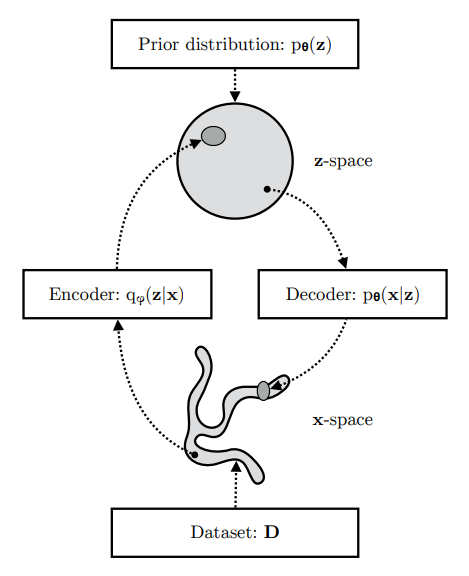
\includegraphics[width=0.75\textwidth]{fig/vae.png}
    \caption{
	VAE learns a stochastic mapping between the observed $ x $-space , whose empirical distribution $ q_D(x) $ is usually complex, and a latent $ z $-space , whose distribution is relatively simple (e.g., a sphere, as shown in the figure). The generative model learns the joint distribution $ p_\theta(x, z) $ which is often (but not always) factorized as: $ p_\theta(x, z) = p_\theta(z) \ p_\theta(x|z) $, with a prior distribution over latent space
	$ p_\theta(z) $, and a stochastic decoder $ p_\theta(x|z) $. The stochastic encoder $ q_\phi(z|x) $, also known as the inference model, approximates the true intractable posterior $ p_\theta(z|x) $ of the generative model.
    }
    \label{fig:vae}
\end{figure}

Consider the following DLVM:
\begin{equation}
\Scale[1.2]{ \displaystyle p_\theta(x) = \int p_\theta(x,z) \,dz }
\end{equation}
For any inference model $ q_\phi(z|x) $ and any variational parameters $ \phi $:
\begin{equation}
\Scale[1.2]{ \displaystyle p_\theta(x) = \int p_\theta(x,z) \frac{q_\phi(z|x)}{q_\phi(z|x)} \,dz }
\end{equation}
Since $ q_\phi(z|x) \approx p_\theta(z|x) $:
\begin{equation}
\Scale[1.2]{ \displaystyle p_\theta(x) = \int p_\theta(x,z) \frac{q_\phi(z|x)}{p_\theta(z|x)} \,dz }
\end{equation}
\begin{equation}
\Scale[1.2]{ \displaystyle p_\theta(x) = \mathbb{E}_{q_\phi(z|x)} \left[ \frac{p_\theta(x,z)}{p_\theta(z|x)} \right] }
\end{equation}
\begin{equation}
\Scale[1.2]{\displaystyle \log p_\theta(x) = \log \mathbb{E}_{q_\phi(z|x)} \left[ \frac{p_\theta(x,z)}{p_\theta(z|x)} \right] }
\end{equation}
The logarithm is a concave function. This can be proven because the second derivative of the logarithm is negative. Therefore, the following holds: $ \log \mathbb{E}_{q_\phi(z|x)} \left[ \frac{p_\theta(x,z)}{p_\theta(z|x)} \right] = \mathbb{E}_{q_\phi(z|x)} \left[ \log \frac{p_\theta(x,z)}{p_\theta(z|x)} \right] $, so that:
\begin{equation}
\Scale[1.2]{\displaystyle \log p_\theta(x) = \mathbb{E}_{q_\phi(z|x)} \left[ \log \frac{p_\theta(x,z)}{p_\theta(z|x)} \right] }
\end{equation}
\begin{equation}
\Scale[1.2]{\displaystyle \log p_\theta(x) = \mathbb{E}_{q_\phi(z|x)} 
\left[ \log \left[ \frac{p_\theta(x,z)}{q_\phi(z|x)} \frac{q_\phi(z|x)}{p_\theta(z|x)} \right] \right] }
\end{equation}
\begin{equation} \label{eq:13}
\Scale[1.2]{\displaystyle \log p_\theta(x) = 
\mathbb{E}_{q_\phi(z|x)} \left[ \log \frac{p_\theta(x,z)}{q_\phi(z|x)} \right]
+
\mathbb{E}_{q_\phi(z|x)} \left[ \log \frac{q_\phi(z|x)}{p_\theta(z|x)} \right]
}
\end{equation}

The second term in Equation (\ref{eq:13}) is the Kullback-Leibler (KL) divergence between $ q_\phi(z|x) $ and $ p_\theta(z|x) $ , which is non-negative:
\begin{equation}
\Scale[1.2]{ \displaystyle \infdiv{q_\phi(z|x)}{p_\theta(z|x)} \geq 0 }
\end{equation}
and equals zero if and only if $ q_\phi(z|x) $ matches the true posterior distribution.
\\

The first term in Equation (\ref{eq:13}) is the variational lower bound, also called the evidence lower bound (ELBO):
\begin{equation}
\Scale[1.2]{ \displaystyle \mathcal{L}_{\theta,\phi}(x) = \mathbb{E}_{q_\phi(z|x)} \left[ \log \frac{p_\theta(x,z)}{q_\phi(z|x)} \right] }
\end{equation}

Since the KL divergence is non-negative, the ELBO serves as a lower bound on the log-likelihood of the data

\begin{equation}
\Scale[1.2]{ \displaystyle \mathcal{L}_{\theta,\phi}(x) = \log p_\theta(x) -  \infdiv{q_\phi(z|x)}{p_\theta(z|x)}}
\end{equation}

\begin{equation}
\Scale[1.2]{ \displaystyle \mathcal{L}_{\theta,\phi}(x) \leq \log p_\theta(x) },
\end{equation}

Thus, Equation (\ref{eq:13}) can be simplified as follows:
\begin{equation}
\Scale[1.2]{\displaystyle \log p_\theta(x) = 
\mathcal{L}_{\theta,\phi}(x)
+
 \infdiv{q_\phi(z|x)}{p_\theta(z|x)}
}
\end{equation}
\begin{equation}
\Scale[1.2]{\displaystyle \log p_\theta(x) \leq 
\log p_\theta(x)
+
 \infdiv{q_\phi(z|x)}{p_\theta(z|x)}
}
\end{equation}


\subsection{DDPM}


We can optimize the log-likelihood using a method similar to VAE. Consider the following DLVM:
\begin{equation}
\Scale[1.2]{ \displaystyle \log p_\theta(x) = \log \int p_\theta(x,z) \,dz }
\end{equation}
\begin{equation}
\Scale[1.2]{ \displaystyle \log p_\theta(x) = \log \int p_\theta(x,z) \frac{q(z|x)}{q(z|x)} \,dz }
\end{equation}
\begin{equation}
\Scale[1.2]{ \displaystyle \log p_\theta(x) = \log \mathbb{E}_{q(z|x)} \left[ \frac{p_\theta(x,z)}{q(z|x)} \right] }
\end{equation}
The logarithm is a concave function. This can be proven because its second derivative is negative. Therefore, the following holds: $ \log \mathbb{E}_{q(z|x)} \left[ \frac{p_\theta(x,z)}{q(z|x)} \right] = \mathbb{E}_{q(z|x)} \left[ \log \frac{p_\theta(x,z)}{q(z|x)} \right] $, , so as:
\begin{equation}
\Scale[1.2]{ \displaystyle \log p_\theta(x) \geq \mathbb{E}_{q(z|x)} \left[\log \frac{p_\theta(x,z)}{q(z|x)} \right] }
\end{equation}

We can apply the same approach to diffusion models. The difference is that the latent variables we use are $ \textbf{x}_{1:T} $  and the observed variable is $ \textbf{x}_0 $. Additionally, instead of directly optimizing a loss function, we seek the expectation of the loss function.
\begin{figure}[h]
    \centering
    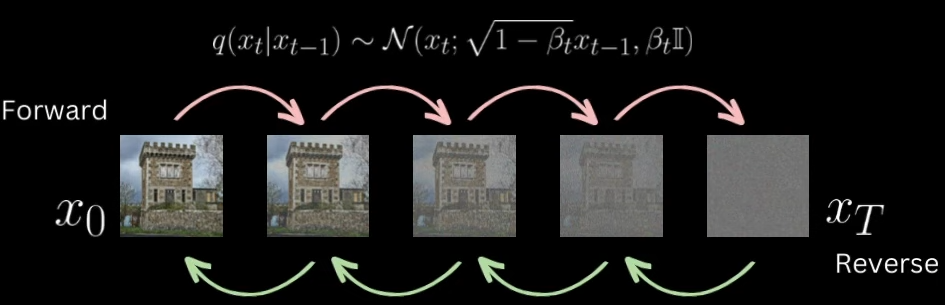
\includegraphics[width=0.5\textwidth]{fig/reverse-process.png}
    \caption{reverse process}
    \label{fig:reverse_process}
\end{figure}

Additionally, instead of maximizing the log-likelihood, we minimize the negative log-likelihood. Essentially, both approaches are equivalent. However, since optimizers typically minimize functions, it is more suitable to use the negative log-likelihood. As the name suggests, a loss function is something we aim to minimize as much as possible.

\begin{equation}
\Scale[1.2]{ \displaystyle \mathbb{E}_{q(\mathbf{x}_0)} \left[ -\log p_\theta(x_0) \right] = 
\mathbb{E}_{q(\mathbf{x}_0)} \left[
-\log \mathbb{E}_{q(\textbf{x}_{1:T}|\textbf{x}_0)} \left[ \frac{p_\theta(\textbf{x}_{0:T})}{q(\textbf{x}_{1:T}|\textbf{x}_0)} \right] \right] }
\end{equation}
\begin{equation}
\Scale[1.2]{ \displaystyle \mathbb{E}_{q(\mathbf{x}_0)} \left[ -\log p_\theta(x_0) \right] \leq
\mathbb{E}_{q(\mathbf{x}_0)} \left[
\mathbb{E}_{q(\textbf{x}_{1:T}|\textbf{x}_0)} \left[ -\log \frac{p_\theta(\textbf{x}_{0:T})}{q(\textbf{x}_{1:T}|\textbf{x}_0)} \right] \right] }
\end{equation}
\begin{equation}
\Scale[1.2]{ \displaystyle \mathbb{E}_{q(\mathbf{x}_0)} \left[ -\log p_\theta(x_0) \right] \leq 
\mathbb{E}_{q(\mathbf{x}_0)} \left[
\mathbb{E}_{q(\textbf{x}_{1:T}|\textbf{x}_0)} \left[ \log \frac{q(\textbf{x}_{1:T}|\textbf{x}_0)}{p_\theta(\textbf{x}_{0:T})} \right] \right] }
\end{equation}
\begin{equation}
\Scale[1.2]{ \displaystyle \mathbb{E}_{q(\mathbf{x}_0)} \left[ -\log p_\theta(x_0) \right] \leq 
\mathbb{E}_{q(\textbf{x}_{0:T})} \left[ \log \frac{q(\textbf{x}_{1:T}|\textbf{x}_0)}{p_\theta(\textbf{x}_{0:T})} \right] }
\end{equation}

Next, we can optimize the term inside the expectation:

\begin{equation}
\Scale[1.2]{ \displaystyle \log \frac{q(\textbf{x}_{1:T}|\textbf{x}_0)}{p_\theta(\textbf{x}_{0:T})} = \log \frac{\displaystyle \prod_{t=1}^{T} q(\textbf{x}_{t}|\textbf{x}_{t-1})}{p(\textbf{x}_T) \displaystyle \prod_{t=1}^{T} p_\theta(\textbf{x}_{t-1}|\textbf{x}_{t})} }
\end{equation}

$ q(\textbf{x}_{t}|\textbf{x}_{t-1}) $ can be rewritten as $ \frac{q(\textbf{x}_{t-1}|\textbf{x}_t) \ q(\textbf{x}_t) }{ q(\textbf{x}_{t-1}) } $. However, $ q(\textbf{x}_{t-1}|\textbf{x}_t) $ will have high variance because there can be multiple candidates for $ \textbf{x}_{t} $.
\begin{figure}[h]
    \centering
    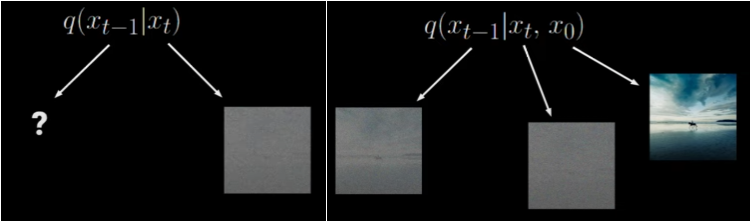
\includegraphics[width=0.75\textwidth]{fig/high-variance-vs-low-variance.png}
    \caption{high variance vs. low variance}
    \label{fig:high-variance-vs-low-variance}
\end{figure}

Therefore, we will introduce the original image $ \textbf{x}_0 $ so that the candidates for $ \textbf{x}_{t-1} $ can better align with the original image.
\begin{equation}
\Scale[1.2]{ \displaystyle \log \frac{q(\textbf{x}_{1:T}|\textbf{x}_0)}{p_\theta(\textbf{x}_{0:T})} = \log \frac{\displaystyle \prod_{t=1}^{T} q(\textbf{x}_{t}|\textbf{x}_{t-1},\textbf{x}_0) } { p(\textbf{x}_T) \displaystyle \prod_{t=1}^{T} p_\theta(\textbf{x}_{t-1}|\textbf{x}_{t})} }
\end{equation}

However, there is something odd. If we examine it more closely, the first term in the numerator contains a self-loop! More precisely, $ q(\textbf{x}_1|\textbf{x}_0,\textbf{x}_0) = \frac{q(\textbf{x}_0|\textbf{x}_1,\textbf{x}_0) \ q(\textbf{x}_1|\textbf{x}_0) }{ q(\textbf{x}_0|\textbf{x}_0) } $. To address this issue, we need to factor out the first term from the product series. Only then can we add $ \textbf{x}_0 $ to the conditional probability in the product series.
\begin{equation}
\Scale[1.2]{ \displaystyle \log \frac{q(\textbf{x}_{1:T}|\textbf{x}_0)}{p_\theta(\textbf{x}_{0:T})} =\xcancel{ \log \frac{\displaystyle \prod_{t=1}^{T} q(\textbf{x}_{t}|\textbf{x}_{t-1},\textbf{x}_0) } { p(\textbf{x}_T) \displaystyle \prod_{t=1}^{T} p_\theta(\textbf{x}_{t-1}|\textbf{x}_{t})} } }
\end{equation}

\begin{equation}
\Scale[1.2]{ \displaystyle \log \frac{q(\textbf{x}_{1:T}|\textbf{x}_0)}{p_\theta(\textbf{x}_{0:T})} = \log \frac{q(\textbf{x}_1|\textbf{x}_0) \displaystyle \prod_{t=2}^{T} q(\textbf{x}_{t}|\textbf{x}_{t-1},\textbf{x}_0) } { p(\textbf{x}_T) \displaystyle \prod_{t=1}^{T} p_\theta(\textbf{x}_{t-1}|\textbf{x}_{t})} }
\end{equation}

\begin{equation}
\Scale[1.2]{ \displaystyle \log \frac{q(\textbf{x}_{1:T}|\textbf{x}_0)}{p_\theta(\textbf{x}_{0:T})} = \log \frac{q(\textbf{x}_1|\textbf{x}_0) \displaystyle \prod_{t=2}^{T} q(\textbf{x}_{t-1}|\textbf{x}_t,\textbf{x}_0) \ q(\textbf{x}_{t}|\textbf{x}_0) } { q(\textbf{x}_{t-1}|\textbf{x}_0) \ p(\textbf{x}_T) \displaystyle \prod_{t=1}^{T} p_\theta(\textbf{x}_{t-1}|\textbf{x}_{t})} }
\end{equation}

\begin{gather}
\nonumber \Scale[1]{ \displaystyle \log \frac{q(\textbf{x}_{1:T}|\textbf{x}_0)}{p_\theta(\textbf{x}_{0:T})} } = \\
\Scale[1]{ \displaystyle \log \frac{ 
\cancel{q(\textbf{x}_1|\textbf{x}_0)}
\ q(\textbf{x}_{T-1}|\textbf{x}_T,\textbf{x}_0) \ q(\textbf{x}_T|\textbf{x}_0) 
\ q(\textbf{x}_{T-2}|\textbf{x}_{T-1},\textbf{x}_0) \ \cancel{q(\textbf{x}_{T-1}|\textbf{x}_0)} 
\ ...
\ q(\textbf{x}_{1}|\textbf{x}_{2},\textbf{x}_0) \ \cancel{q(\textbf{x}_{2}|\textbf{x}_0)} 
} 
{ 
\cancel{q(\textbf{x}_{T-1}|\textbf{x}_0)} 
\ q(\textbf{x}_{T-2}|\textbf{x}_0)
\ ...
\ \cancel{q(\textbf{x}_{2}|\textbf{x}_0)}
\ \cancel{q(\textbf{x}_{1}|\textbf{x}_0)}
\ p(\textbf{x}_T) \displaystyle \prod_{t=1}^{T} p_\theta(\textbf{x}_{t-1}|\textbf{x}_{t}) } }
 \end{gather}

\begin{equation}
\Scale[1.2]{ \displaystyle \log \frac{q(\textbf{x}_{1:T}|\textbf{x}_0)}{p_\theta(\textbf{x}_{0:T})} = \log \frac{
q(\textbf{x}_T|\textbf{x}_0) \displaystyle \prod_{t=2}^{T} q(\textbf{x}_{t-1}|\textbf{x}_t,\textbf{x}_0)
} 
{ 
p(\textbf{x}_T) \displaystyle \prod_{t=1}^{T} p_\theta(\textbf{x}_{t-1}|\textbf{x}_{t})
} }
\end{equation}

\begin{equation}
\Scale[1.2]{ \displaystyle \log \frac{q(\textbf{x}_{1:T}|\textbf{x}_0)}{p_\theta(\textbf{x}_{0:T})} = \log \frac{
q(\textbf{x}_T|\textbf{x}_0) \displaystyle \prod_{t=2}^{T} q(\textbf{x}_{t-1}|\textbf{x}_t,\textbf{x}_0)
} 
{ 
p(\textbf{x}_T) \ p_\theta(\textbf{x}_0|\textbf{x}_1) \displaystyle \prod_{t=2}^{T} p_\theta(\textbf{x}_{t-1}|\textbf{x}_{t})
} }
\end{equation}

\begin{equation}
\Scale[1.2]{ \displaystyle \log \frac{q(\textbf{x}_{1:T}|\textbf{x}_0)}{p_\theta(\textbf{x}_{0:T})} = \log \frac{
q(\textbf{x}_T|\textbf{x}_0)
} 
{ 
p(\textbf{x}_T)
} + 
\sum_{t=2}^{T} \log \frac{
q(\textbf{x}_{t-1}|\textbf{x}_t,\textbf{x}_0)
}
{
p_\theta(\textbf{x}_{t-1}|\textbf{x}_{t})
} -
\log p_\theta(\textbf{x}_0|\textbf{x}_1)
}
\end{equation}

Reinsert $ \log \frac{q(\textbf{x}_{1:T}|\textbf{x}_0)}{p_\theta(\textbf{x}_{0:T})} $  into the loss function:
\begin{equation}
\Scale[1.2]{ \displaystyle \mathbb{E}_{ q(\textbf{x}_{0}) } \left[ -\log p_\theta(\textbf{x}_0) \right] \leq \mathbb{E}_{ q(\textbf{x}_{0:T}) } \left[ 
\log \frac{
q(\textbf{x}_T|\textbf{x}_0)
} 
{ 
p(\textbf{x}_T)
} + 
\sum_{t=2}^{T} \log \frac{
q(\textbf{x}_{t-1}|\textbf{x}_t,\textbf{x}_0)
}
{
p_\theta(\textbf{x}_{t-1}|\textbf{x}_{t})
} -
\log p_\theta(\textbf{x}_0|\textbf{x}_1)
\right]. }
\end{equation}

Convert each term in the loss function into the form of KL (Kullback–Leibler) divergence:
\begin{equation}
\Scale[1.2]{ \displaystyle
\mathbb{E}_{q(\textbf{x}_{0:T})} \left[ 
\log \frac{
q(\textbf{x}_T|\textbf{x}_0)
} 
{ 
p(\textbf{x}_T)
} + 
\sum_{t=2}^{T} \log \frac{
q(\textbf{x}_{t-1}|\textbf{x}_t,\textbf{x}_0)
}
{
p_\theta(\textbf{x}_{t-1}|\textbf{x}_{t})
} -
\log p_\theta(\textbf{x}_0|\textbf{x}_1)
\right] 
}
\end{equation}

\begin{equation}
\Scale[1.2]{ \displaystyle = 
\mathbb{E}_{q(\textbf{x}_{0:T})} \left[ 
\infdiv{q(\textbf{x}_T|\textbf{x}_0)}{p(\textbf{x}_T)}
+ 
\sum_{t=2}^{T} \infdiv{ 
q(\textbf{x}_{t-1}|\textbf{x}_t,\textbf{x}_0)
}
{
p_\theta(\textbf{x}_{t-1}|\textbf{x}_{t})
}
-
\log p_\theta(\textbf{x}_0|\textbf{x}_1)
\right]
}
\end{equation}

We get:
\begin{equation}
\Scale[1.2]{ \displaystyle
{\small L = 
\mathbb{E}_{q(\textbf{x}_{0:T})} \left[ 
\infdiv{q(\textbf{x}_T|\textbf{x}_0)}{p(\textbf{x}_T)}
+ 
\sum_{t=2}^{T} \infdiv{ 
q(\textbf{x}_{t-1}|\textbf{x}_t,\textbf{x}_0)
}
{
p_\theta(\textbf{x}_{t-1}|\textbf{x}_{t})
}
-
\log p_\theta(\textbf{x}_0|\textbf{x}_1)
\right]
} }
\end{equation}

with
 
\begin{equation}
\Scale[1.2]{ \displaystyle
q(\textbf{x}_{t-1}|\textbf{x}_t,\textbf{x}_0) = \mathscr{N}(\textbf{x}_{t-1};\tilde{\mu}_t(\textbf{x}_{t},\textbf{x}_0),\tilde{\beta}_t\textbf{I}), }
\end{equation}

\begin{equation}
\Scale[1.2]{ \displaystyle
\tilde{\mu}_t(\textbf{x}_{t},\textbf{x}_0) \coloneq \frac{
\sqrt{\bar{\alpha}_{t-1}}\beta_t
}
{
1 - \bar{\alpha}_t
}
\textbf{x}_0 
+
\frac{
\sqrt{\alpha_{t}}(1-\bar{\alpha}_{t-1})
}
{
1 - \bar{\alpha_t}
}
\textbf{x}_t, }
\end{equation}

\begin{equation}
\Scale[1.2]{ \displaystyle
\tilde{\beta}_t \coloneq 
\frac{
1-\bar{\alpha}_{t-1}
}
{
1-\bar{\alpha}
}
\beta_t. }
\end{equation}

We can decompose $ L $ into:
\begin{equation}
\Scale[1.2]{ \displaystyle
L_T = 
\infdiv{q(\textbf{x}_T|\textbf{x}_0)}{p(\textbf{x}_T)}. }
\end{equation}

\begin{equation}
\Scale[1.2]{ \displaystyle
L_{t-1} = 
\infdiv{ 
q(\textbf{x}_{t-1}|\textbf{x}_t,\textbf{x}_0)
}
{
p_\theta(\textbf{x}_{t-1}|\textbf{x}_{t})
}. }
\end{equation}

\begin{equation}
\Scale[1.2]{ \displaystyle
L_{0} = 
\log p_\theta(\textbf{x}_0|\textbf{x}_1). }
\end{equation}


\subsection{Forward process and $ L_T $}
In fact, $ \beta_t $ can be learned through reparameterization. However, the value of $ \beta_t $ is kept constant, meaning that $ q $ has no learnable parameters. This makes $ L_T $ constant during training and therefore can be ignored.


\subsection{Reverse process and $ L_{1:T-1} $}
We aim to learn the mean and variance of the reverse diffusion process $ p_\theta(\textbf{x}_{t-1}|\textbf{x}_{t}) = \mathscr{N}(\textbf{x}_{t-1};\mu_\theta(\textbf{x}_{t},t),\Sigma_\theta(\textbf{x}_t, t)) $, where $ 1 < t < T  $. Here, the authors decided not to learn the variance and instead set it as a constant
\begin{equation}
\Scale[1.2]{ \displaystyle
\Sigma_\theta(\textbf{x}_t, t) = \sigma_t^2 \textbf{I} }
\end{equation}

, so that

\begin{equation}
\Scale[1.2]{ \displaystyle
 p_\theta(\textbf{x}_{t-1}|\textbf{x}_{t}) = \mathscr{N}(\textbf{x}_{t-1};\mu_\theta(\textbf{x}_{t},t),\sigma_t^2 \textbf{I}) }
\end{equation}

To represent the mean $ \mu_\theta(\textbf{x}_{t},t) $, the DDPM authors parameterized it based on the analysis of $ L_t $, namely $
\infdiv{ 
q(\textbf{x}_{t}|\textbf{x}_{t+1},\textbf{x}_0)
}
{
p_\theta(\textbf{x}_{t}|\textbf{x}_{t+1})
}
$, using the mean square error:

\begin{equation}
\Scale[1.2]{ \displaystyle
L_{t-1} = \mathbb{E}_{q} \left[ 
\frac{1}{2\sigma_t^2}
\norm{
\tilde{\mu}_t(\textbf{x}_{t},\textbf{x}_0) - \mu_\theta(\textbf{x}_{t},t)
}^2
\right] + C, }
\end{equation}

with C being a constant that does not depend on $ \theta $. Substitute $ \tilde{\mu}_t(\textbf{x}_{t},\textbf{x}_0) $ into (12):

\begin{equation}
\Scale[1.2]{ \displaystyle
L_{t-1} = \mathbb{E}_{q} \left[ 
\frac{1}{2\sigma_t^2}
\norm{
\frac{
\sqrt{\bar{\alpha}_{t-1}}\beta_t
}
{
1 - \bar{\alpha}_t
}
\textbf{x}_0 
+
\frac{
\sqrt{\alpha_{t}}(1-\bar{\alpha}_{t-1})
}
{
1 - \bar{\alpha_t}
}
\textbf{x}_t 
-
 \mu_\theta(\textbf{x}_{t},t)
}^2
\right] + C, }
\end{equation}

In equation (2), we have seen how to find $ \textbf{x}_t $ given $ \textbf{x}_0 $. We can use that equation to find $ \textbf{x}_0 $:
\begin{equation}
\Scale[1.2]{ \displaystyle
\textbf{x}_t = \sqrt{\bar{\alpha_t}} \textbf{x}_{0} + \sqrt{1-\bar{\alpha_t}} \epsilon}
\end{equation}

\begin{equation}
\Scale[1.2]{ \displaystyle
\iff \textbf{x}_0 = \frac{1}{\sqrt{\bar{\alpha_t}}}(\textbf{x}_{t} - \sqrt{1-\bar{\alpha}_t} \epsilon) }
\end{equation}

Substitute $ \textbf{x}_0 $ into (14):

\begin{equation}
\Scale[1.2]{ \displaystyle
L_{t-1} = \mathbb{E}_{q} \left[ 
\frac{1}{2\sigma_t^2}
\norm{
\frac{
\sqrt{\bar{\alpha}_{t-1}}\beta_t
}
{
1 - \bar{\alpha}_t
}
\frac{1}{\sqrt{\bar{\alpha_t}}}(\textbf{x}_{t} - \sqrt{1-\bar{\alpha}_t} \epsilon)
+
\frac{
\sqrt{\alpha_{t}}(1-\bar{\alpha}_{t-1})
}
{
1 - \bar{\alpha_t}
}
\textbf{x}_t 
-
\mu_\theta(\textbf{x}_{t},t)
}^2
\right] + C }
\end{equation}

\begin{equation}
\Scale[1.2]{ \displaystyle
\hspace{2em} = \mathbb{E}_{q} \left[ 
\frac{1}{2\sigma_t^2}
\norm{
\frac{1}{\sqrt{\bar{\alpha}_t}}(\textbf{x}_t - \frac{\beta_t}{\sqrt{1-\bar{\alpha}_t}} \epsilon)
-
\mu_\theta(\textbf{x}_{t},t)
}^2
\right] + C 
}
\end{equation}

The authors of DDPM reparameterize $ x_t $ to predict the noise in the reverse diffusion process:
\begin{equation}
\Scale[1.2]{ \displaystyle
\hspace{2em} = \mathbb{E}_{q} \left[ 
\frac{1}{2\sigma_t^2}
\norm{
\frac{1}{\sqrt{\bar{\alpha}_t}} ( \textbf{x}_t(\textbf{x}_0,\epsilon ) - \frac{\beta_t}{\sqrt{1-\bar{\alpha}_t}} \epsilon)
-
\mu_\theta(\textbf{x}_t(\textbf{x}_0,\epsilon),t)
}^2
\right] + C, }
\end{equation}

with $ \textbf{x}_t(\textbf{x}_0,\epsilon) = \sqrt{\bar{\alpha}_t}\textbf{x}_0 + \sqrt{1-\bar{\alpha}_t}\epsilon, \hspace{1em} \epsilon \sim\mathscr{N}(0,\textbf{I}). $
Equation (10) shows that $ \mu_\theta $ must predict $ \frac{1}{\sqrt{\bar{\alpha}_t}} ( \textbf{x}_t(\textbf{x}_0,\epsilon ) - \frac{\beta_t}{\sqrt{1-\bar{\alpha}_t}} \epsilon) $, given $ \textbf{t} $. Since $ \textbf{t} $ is already included as an input, we can parameterize it as follows:

\begin{equation}
\Scale[1.2]{ \displaystyle
\mu_\theta(\textbf{x}_{t},t) = \bar{\mu}_t(\textbf{x}_{t}, \textbf{x}_0(\textbf(x)_t, \epsilon_\theta)) }
\end{equation}

\begin{equation}
\Scale[1.2]{ \displaystyle
\hspace{2em} = \bar{\mu}_t(\textbf{x}_{t}, \frac{1}{\sqrt{\bar{\alpha_t}}}(\textbf{x}_{t} - \sqrt{1-\bar{\alpha}_t} \epsilon_\theta(\textbf{x}_t))) }
\end{equation}

\begin{fleqn}[\parindent]
\begin{equation}
\begin{split}
\hspace{2.25em} = \frac{1}{\sqrt{\bar{\alpha}_t}} ( \textbf{x}_t - \frac{\beta_t}{\sqrt{1-\bar{\alpha}_t}} \epsilon_\theta(\textbf{x}_t, t))
\end{split}
\end{equation}
\end{fleqn}

Substitute Equation (16) into Equation (15):
\begin{equation}
\Scale[1.2]{ \displaystyle
L_{t-1} = \mathbb{E}_{q} \left[ 
\frac{1}{2\sigma_t^2}
\norm{
\frac{1}{\sqrt{\bar{\alpha}_t}} ( \textbf{x}_t - \frac{\beta_t}{\sqrt{1-\bar{\alpha}_t}} \epsilon)
-
\mu_\theta(\textbf{x}_t,t)
}^2
\right] + C }
\end{equation}

\begin{equation}
\Scale[1.2]{ \displaystyle
\hspace{2.25em} = \mathbb{E}_{q} \left[ 
\frac{1}{2\sigma_t^2}
\norm{
\frac{1}{\sqrt{\bar{\alpha}_t}} ( \textbf{x}_t - \frac{\beta_t}{\sqrt{1-\bar{\alpha}_t}} \epsilon)
-
\frac{1}{\sqrt{\bar{\alpha}_t}} ( \textbf{x}_t - \frac{\beta_t}{\sqrt{1-\bar{\alpha}_t}} \epsilon_\theta(\textbf{x}_t, t))
}^2
\right] + C }
\end{equation}

\begin{fleqn}[\parindent]
\begin{equation}
\begin{split}
\hspace{2.25em} = \mathbb{E}_{q} \left[ 
\frac{\beta_t^2}{2\sigma_t^2\alpha_t(1-\bar{\alpha}_t)}
\norm{
\epsilon
-
\epsilon_\theta(\textbf{x}_t, t)
}^2
\right] + C
\end{split}
\end{equation}
\end{fleqn}

After conducting experiments, the DDPM authors found that removing the first term in (17) during training improves sample quality and makes implementation easier.
\begin{equation}
\Scale[1.2]{ \displaystyle
L_{simple}(\theta) \coloneq \mathbb{E}_{q} \left[ 
\norm{
\epsilon
-
\epsilon_\theta(\textbf{x}_t, t)
}^2
\right] }
\end{equation}

Recall that $ p_\theta(\textbf{x}_{t-1}|\textbf{x}_{t}) = \mathscr{N}(\textbf{x}_{t-1};\mu_\theta(\textbf{x}_{t},t),\Sigma_\theta(\textbf{x}_t, t)) $, we can sample $ \textbf{x}_{t-1} $ using the reparameterization trick $ \mathscr{N}(\mu,\sigma^2) = \mu + \sigma \epsilon $:
\begin{equation}
\Scale[1.2]{ \displaystyle
\textbf{x}_{t-1} = \mu_\theta(\textbf{x}_{t},t) + \Sigma_\theta(\textbf{x}_{t},t) + \epsilon }
\end{equation}

\begin{fleqn}[\parindent]
\begin{equation}
\begin{split}
\hspace{2.25em} = \frac{1}{\sqrt{\bar{\alpha}_t}} ( \textbf{x}_t - \frac{\beta_t}{\sqrt{1-\bar{\alpha}_t}} \epsilon_\theta(\textbf{x}_t, t)) + \sqrt{\beta_t} \epsilon
\end{split}
\end{equation}
\end{fleqn}


\section{Data Scaling}


\end{document}